\documentclass[letter, 11pt]{article}
%% ================================
%% Packages =======================
\usepackage[utf8]{inputenc}      %%
\usepackage[T1]{fontenc}         %%
\usepackage{lmodern}             %%
\usepackage[spanish]{babel}      %%
\decimalpoint                    %%
\usepackage{fullpage}            %%
\usepackage{fancyhdr}            %%
\usepackage{graphicx}            %%
\usepackage{amsmath}             %%
\usepackage{amssymb}             %%
\usepackage{color}               %%
\usepackage{mdframed}            %%
\usepackage[colorlinks]{hyperref}%%
%% ================================
%% ================================

%% ================================
%% Page size/borders config =======
\setlength{\oddsidemargin}{0in}  %%
\setlength{\evensidemargin}{0in} %%
\setlength{\marginparwidth}{0in} %%
\setlength{\marginparsep}{0in}   %%
\setlength{\voffset}{-0.5in}     %%
\setlength{\hoffset}{0in}        %%
\setlength{\topmargin}{0in}      %%
\setlength{\headheight}{54pt}    %%
\setlength{\headsep}{1em}        %%
\setlength{\textheight}{8.5in}   %%
\setlength{\footskip}{0.5in}     %%
%% ================================
%% ================================

%% =============================================================
%% Headers setup, environments, colors, etc.
%%
%% Header ------------------------------------------------------
\fancypagestyle{firstpage}
{
  \fancyhf{}
  \lhead{
\includegraphics[height=4.5em]{../LogoDFI.jpg}}
  \rhead{FI3104-1 \semestre\\
         Métodos Numéricos para la Ciencia e Ingeniería}
  \fancyfoot[C]{\thepage}
}

\pagestyle{plain}
\fancyhf{}
\fancyfoot[C]{\thepage}
%% -------------------------------------------------------------
%% Environments -------------------------------------------------
\newmdenv[
  linecolor=gray,
  fontcolor=gray,
  linewidth=0.2em,
  topline=false,
  bottomline=false,
  rightline=false,
  skipabove=\topsep
  skipbelow=\topsep,
]{ayuda}
%% -------------------------------------------------------------
%% Colors ------------------------------------------------------
\definecolor{gray}{rgb}{0.5, 0.5, 0.5}
%% -------------------------------------------------------------
%% Aliases ------------------------------------------------------
\newcommand{\scipy}{\texttt{scipy}}
%% -------------------------------------------------------------
%% =============================================================

%% =============================================================================
%% CONFIGURACION DEL DOCUMENTO =================================================
%% Llenar con la información pertinente al curso y la tarea
%%
\newcommand{\fechaentrega}{XX/XX/XXXX XX:XX hrs}
\newcommand{\semestre}{201XB}
%% =============================================================================
%% =============================================================================


\begin{document}
\thispagestyle{firstpage}

\begin{center}
  {\uppercase{\LARGE \bf Informe Tarea XX}}
\end{center}

\noindent{\Large Valentino González}\\
\noindent{\Large RUT:XX.XXX.XXX-X}\\
\noindent{\Large Github: @thevalentino}


%% =============================================================================
%% =============================================================================
\section{Introducción}

El objetivo de esta tarea es encontrar el valor de $a$ que resuelve la Ecuación
(1) del enunciado. Si $x$ es una variable aleatoria sacada de la distribución
descrita en el enunciado, entonces $a$ representa un valor que asegura que los
valores aleatorios de $x$ serán mayores que $a$ solo un 5\% de las veces.

\begin{equation}
0.05 = \int_{a}^{\infty} \frac{1}{\sqrt{2\pi}} \exp\left({\frac{-y^2}{2}}\right) dy
\end{equation}

La ecuación a resolver incluye el cálculo de una integral que debe ser
regularizada pues sus límites van de $0$ a $\infty$. Implementaremos un cambio
de variable que regulariza los límites y luego una función que calcule la
integral de forma numérica para resolverla para distintos valores de $a$.

Finalmente implementaremos una función que busque el valor de $a$ que hace que la
integral original valga 0.05.

\section{Desarrollo}

Lo primero es regularizar la integral. Para ello seguimos la sugerencia del
enunciado y aplicamos el cambio de variable $u=1/y$, con lo que el problema se
transforma en:

\begin{equation}
0.05 = \int_0^{1/a} \frac{1}{\sqrt{2\pi}u^2} \exp\left({\frac{-1}{2u^2}}\right) du
\end{equation}

La forma de la función a integrar se puede apreciar en la Figura 1. Llamaremos
a esta función $f(u)$.

\begin{figure}[!ht]
  \centering
  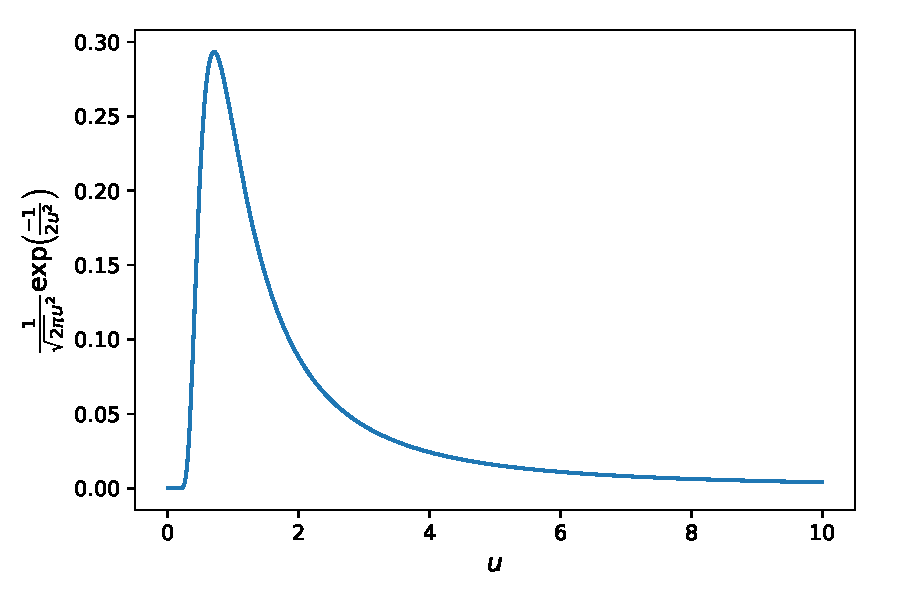
\includegraphics[height=8cm]{../solucion/integral.pdf}
  \caption{La función que vamos a integrar.}
\end{figure}

Para integrar $f(u)$ utilizaremos la función \texttt{scipy.interpolate.quad},
la cual es una implementación de la librería \texttt{QUADPACK} escrita en
\texttt{FORTRAN}. Esta librería implementa el método de {\it cuadratura
adaptativa} e intenta automáticamente escoger el algoritmo necesario para
calcular la integral con una precisión dada por el usuario. Para más
información: https://en.wikipedia.org/wiki/QUADPAC

Definimos entonces la función:

\begin{equation}
  I(a) =  \int_0^{1/a} \frac{1}{\sqrt{2\pi}u^2} \exp\left({\frac{-1}{2u^2}}\right) du
\end{equation}

cuya forma se muestra en la Figura (2). $I(a)$ se calcula numéricamente con la
función \texttt{quad} con sus parámetros por defecto. Los más importantes son
las tolerancias absoluta y relativa: {\it epsabs=1.49e-08, epsrel=1.49e-08}, y
el límite máximo de sub-intervalos para el algoritmo adaptativo: {\it
limit=50}.

Es importante notar que la función $f(u)$ se indefine en $u=0$. Sin embargo,
como se aprecia en la Figura (1), el área bajo la curva en las cercanías de
cero pequeña por, lo que podríamos partir la integral en algún valor $\epsilon
\gtrsim 0$. El algoritmo de \texttt{quad} es capaz de manejar esta indefinición
automáticamente, por lo que no implementamos ningún cambio relacionado a la
indefinición de la función $f(u)$.

\begin{figure}[!hb]
  \centering
  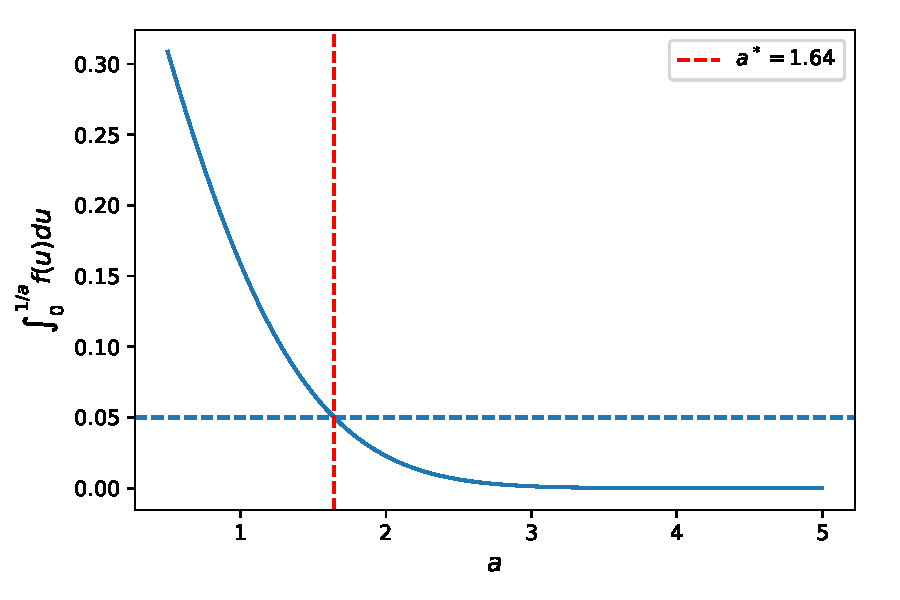
\includegraphics[height=8cm]{../solucion/solucion.pdf}
  \caption{La función $I(a)$. Buscamos el valor de $a$ para el cual la función
  toma el valor 0.05 (linea azul horizontal punteada). Utilizando el algoritmo
de newton, encontramos la solución $a^*=1.64$ (línea roja vertical punteada).}
\end{figure}

Finalmente, es necesario resolver la ecuación:

\begin{equation}
  I(a^*) - 0.05 = 0
\end{equation}

Esto lo hacemos utilizando el método de newton (en realidad de la secante),
implementado en \texttt{scipy.optimize.newton}. Utilizamos los parámetros por
defecto, en particular, la tolerancia absoluta {\it tol=1.48e-08} y el número
máximo de iteraciones {\it maxiter=50}. Le damos como punto de partida el valor
$a_0=1$. El algoritmo converge luego de $7$ iteraciones encontrando el valor
$a^*= 1.64485363$.

Otros valores del punto de partida convergen a un valor muy cercano con
diferencias en el número de iteraciones necesarias. Por ejemplo para $a_0=0.5$,
el algoritmo converge luego de 8 iteraciones.

\section{Discusión y Conclusiones}

Si $x$ es una variable aleatoria sacada de una gausiana con parámetros $\mu=0$
y $\sigma=1$, entonces sólo tomará valores mayores a $a^*=1.64$ el 5\% de las
veces.

Si bien este problema involucra el cálculo de una integral de límites
indefinidos (Ecuación 1), el cambio de variable $u = 1/y$ resulta en una
función bien comportada. En particular, la suavidad de la función (ver Figura
2), asegura que algoritmos como el de la {\it secante} para buscar raíces
converjan de manera robusta (casi independiente del punto de partida elegido),
y en pocas [sic.] iterasiones.



\end{document}
